\documentclass{beamer}
\mode<presentation>{}

\graphicspath{ {./figures/} }
\usepackage{enumitem,xcolor}
\usepackage{tikz}
\usetikzlibrary{shadows,arrows.meta,positioning,backgrounds,fit}
\usepackage{subcaption}
\usepackage{fontawesome5} %% nice little symbols ...
\usepackage{natbib} %% for bibliography
%\bibliographystyle{plainnat}
\bibliographystyle{apalike}

%\setbeamertemplate{footline}[frame number]
%\setbeamertemplate{headline}{}
\setbeamertemplate
 {footline}{\quad\hfill\insertframenumber/\inserttotalframenumber\strut\quad}

% colored underline, with Beamer overlay support
% usage: \cul{x} or \cul[blue]{x} or \cul<2->{x} or \cul<2->[blue]{x}
\newcommand<>{\cul}[2][red]{%
  % change underline dimentions: https://tex.stackexchange.com/a/167957/25264
  \fontdimen6\textfont3=0.75pt%
  % colored underline: https://tex.stackexchange.com/a/9477/25264
  % transparent underline: https://tex.stackexchange.com/a/45601/25264
  % switch between colored and transparent: http://mirrors.ibiblio.org/CTAN/macros/latex/contrib/beamer/doc/beameruserguide.pdf sections 9.3 and 9.6.1
  \alt#3%
      {\color{#1}\underline{{\color{black}#2}}\color{black}}%
      {\transparent{0.0}\underline{{\transparent{1.0}#2}}\transparent{1.0}} %
}

% so that the captions are numerated
\setbeamertemplate{caption}[numbered]

% when issuing \appendinx in the deocument, these extra slides will not be 
% counted
\renewcommand{\appendixname}{\texorpdfstring{\translate{Appendix}}{Appendix}}

%% Tikz Stuff
% Define block styles
\tikzset{%
  materia/.style={draw, fill=blue!10, text width=4.0em, text centered, minimum height=1.5em,drop shadow},
  etape/.style={materia, text width=6em, minimum width=7em, minimum height=2em, rounded corners, drop shadow},
  texto/.style={above, text width=4em, text centered},
  linepart/.style={draw, thick, color=black!50, -LaTeX, dashed},
  line/.style={draw, thick, color=black!50, -LaTeX},
  ur/.style={draw, text centered, minimum height=0.01em},
  back group/.style={fill=yellow!20,rounded corners, draw=black!50, dashed, inner xsep=15pt, inner ysep=10pt},
}
\newcommand{\etape}[2]{node (p#1) [etape] {#2}}
\newcommand{\transreceptor}[4]{%
  \path [linepart] (#1.#4) -- node [above] {\scriptsize \textcolor{red!40}{#2}} (#3);}
%% DOne with Tikz stuff !!

%% For verbatim
\newenvironment{VerbExample}
{\semiverbatim}
{\endsemiverbatim}

\title{Progress Report and Lessons Learned from Developing a DORIS POD Software}
\author{X. ~Papanikolaou\inst{1} \and M. ~Tsakiri\inst{1} 
  \and S. ~Nahmani\inst{2} \and A. ~Pollet\inst{2} 
  \and D. ~Anastasiou\inst{1} \and V. ~Zacharis\inst{1}}
\institute
{
  \inst{1}%
  Dionysos Satellite Observatory\\
  School of Rural, Surveying \& Geoinformatics Engineering\\
  National Technical University of Athens
  \and
  \inst{2}%
  Institut de Physique du Globe de Paris\\
  Université Paris Cité
}

\date{{\color{red!30} IDS Workshop,\\ 
  30 Years of Progress in Radar Altimetry Symposium,\\
  2-7 September 2024, Montpellier, France}}

% Top left and top right  Position of a logo in beamer
\titlegraphic {
\begin{tikzpicture}[overlay,remember picture]
\node[right=0.2cm] at (current page.150){
    \includegraphics[width=1cm]{DSOtrans}
  };
\node[left=0.2cm] at (current page.30){
    \includegraphics[width=1cm]{ntua}
  };
\end{tikzpicture}
}

\begin{document}
  
\parskip=10pt

\begin{frame}[noframenumbering, plain]
  \titlepage
\end{frame}

\begin{frame}{}
\frametitle{Dionysos DORIS Beacon}
Dionysos Satellite Observatory (DSO) has been hosting a DORIS beacon in its 
facilities since 1989. First setup equipped with an \texttt{Alcatel} antenna, 
upgraded in May 2006 to \texttt{Starec} (\ref{fig:diob}).
\begin{figure}
  \centering
  \begin{subfigure}[t]{0.45\textwidth}
    \includegraphics[width=1\textwidth]{DIOB_202103}
    \caption{DORIS Beacon DIOB (Starec)}
    \label{fig:diob}
  \end{subfigure}
  \begin{subfigure}[t]{0.45\textwidth}
    \includegraphics[width=1.1\textwidth]{dso_fire}
    %\caption{DORIS Beacon DIOA (Alcatel)}
    \caption{That was close \dots}
    \label{fig:dioa}
  \end{subfigure}
  %\caption{DORIS beacon hosted hosted at DSO facilities}
  \label{fig:dioa-and-diob}
\end{figure}
\end{frame}

\begin{frame}{Background}
\frametitle{Involvement in IDS \& Motivation}
  Since late 2021, DSO has decided to expand its involvement in the 
  DORIS community by developing its own, in-house processing software for 
  POD and positioning using the DORIS system.

  The software is designed and build \cul[red!40]{from scratch}, adopting 
  recent developments in DORIS analysis and Satellite Geodesy.
\begin{itemize}[label=\textcolor{blue!40}{\textbullet}]
  \item expand out knowledge-base and expertise (research activity \& academic 
    services),
  \item follow and apply state-of-the-art technologies in Satellite Geodesy 
    and expand \& modernize our research activity,
  \item contribute to the DORIS/IDS community, and get involved ongoing/future 
    projects
\end{itemize}
\end{frame}

\begin{frame}{}
\frametitle{Plan Outline}
Our goal is to develop a DORIS \cul[red!40]{free and open-source} analysis 
software for POD \& positioning.

We follow an incremental approach, integrating one component at a time. As a 
first step, we are targeting:
\begin{itemize}
  \item [\textcolor{blue!40}{\textbullet}] (P)OD-only
  \begin{itemize}
    \item [\textcolor{blue!40}{\textbullet}] Jason-3 satellite
      \begin{itemize}
        \item [\textcolor{blue!40}{\textbullet}] adopt \& implement simple 
          models initially; \textcolor{red!40}{gradually increase complexity}
       \end{itemize}
    \item [\textcolor{green!40}{\checkmark}] \textcolor{red!40}{gradually incorporate more 
      satellites \ldots}
  \end{itemize}
  \item [\textcolor{green!40}{\checkmark}] introduce positioning once POD is 
    acceptable
\end{itemize}
\end{frame}

\begin{frame}
  \frametitle{Workflow}
    \framesubtitle{Development Plan \& Milestones}
  \begin{figure}
  \centering
  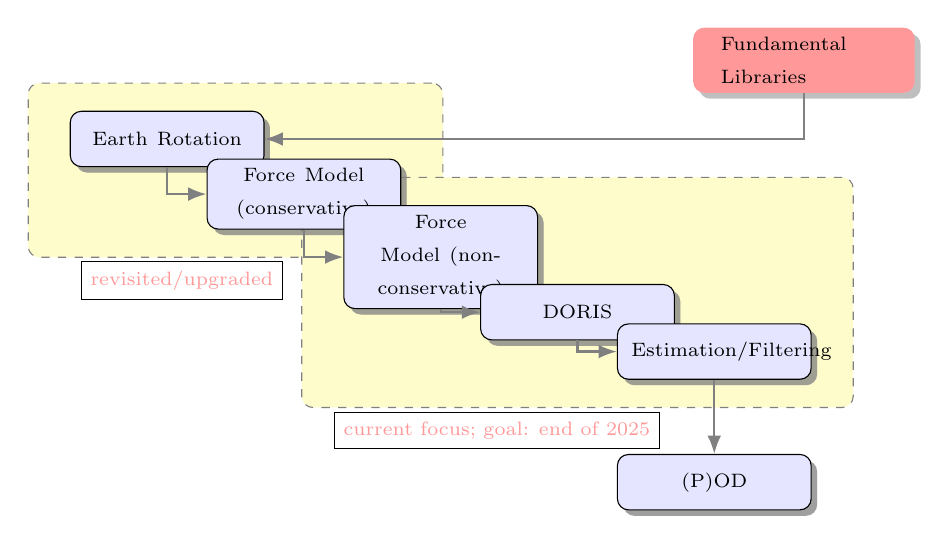
\begin{tikzpicture}
    %\etape{1}{Fundamental libraries};
    \node[fill=red!40, text width=6em, minimum width=8em, minimum height=2em, rounded corners, drop shadow] at (0, 0) (p1) {\scriptsize Fundamental Libraries};
    \path (p1.east)+(-9.5, -1.0) \etape{2}{\scriptsize Earth Rotation};
    \path (p2.east)+(+0.5, -0.7) \etape{3}{\scriptsize Force Model (conservative)};
    \path (p3.east)+(+0.5, -0.8) \etape{4}{\scriptsize Force Model (non-conservative)};
    \path (p4.east)+(+0.5, -0.7) \etape{5}{\scriptsize DORIS};
    \path (p5.east)+(+0.5, -0.5) \etape{6}{\scriptsize Estimation/Filtering};
    \path (p6.south)+(+0.0, -1.3) \etape{7}{\scriptsize (P)OD};
  
    \path [line] (p1.south) |- node [above] {} (p2);
    \path [line] (p2.south) |- node [above] {} (p3.west);
    \path [line] (p3.south) |- node [above] {} (p4.west);
    \path [line] (p4.south) |- node [above] {} (p5.west);
    \path [line] (p5.south) |- node [above] {} (p6.west);
    \path [line] (p6.south) -- node [above] {} (p7.north);
  
    \begin{scope}[on background layer]
      \node (bk1) [back group] [fit=(p2) (p3)] {};
      \node (bk2) [back group] [fit=(p4) (p6)] {};
      %\node (bk3) [back group] [fit=(p3) (p7)] {};
    %  \node [draw, thick, green!50!black, fill=green!75!black!25, rounded corners, fit=(p1), inner xsep=15pt, inner ysep=10pt] {};
    \end{scope}
  
    \node[draw] at (-7.9,-2.8) {\scriptsize \textcolor{red!40}{revisited/upgraded}};
    \node[draw] at (-3.9,-4.7) {\scriptsize \textcolor{red!40}{current focus; goal: end of 2025}};

  \end{tikzpicture}
  \end{figure}
\end{frame}

\begin{frame}{}
\frametitle{Phase-I Results}
\begin{figure}
  \centering
  \begin{subfigure}[t]{0.45\textwidth}
    \includegraphics[width=1\textwidth]{t5statediffs}
    \caption{State differences w.r.t CNES/SSALTO orbits, Jason-3.}
    \label{fig:state-diffs-xyz}
  \end{subfigure}
  \begin{subfigure}[t]{0.50\textwidth}
    \includegraphics[width=1.1\textwidth]{t5resVsEleVsAntenna}
    \caption{Residuals w.r.t Elevation, per antenna type.}
    \label{fig:state-diffs-rtn}
  \end{subfigure}
  \caption{Periminary results for Jason-3, at 05/09/2022}
  \label{fig:state-diffs}
\end{figure}
\end{frame}

\begin{frame}
  \frametitle{Design Considerations (1/2)}
  \begin{itemize}[label=\textcolor{blue!40}{\textbullet}]
    \item Core software development using the \textbf{C++} 
      programming language (exploiting its speed, robustness \& versatility)
    \item Various minor, peripheral parts developed using \textbf{Python}, 
      allowing development speed and ease of use (for developers \& users)
    \item Follow a \textbf{\emph{modular}} design pattern, with different 
      parts developed individually, serving specific needs, thus favoring 
      composability \& reusability
    \item Strive for \textbf{minimum dependencies}; when unavoidable, we 
      only use open-source software
    \item Developed in an ``\textbf{open}'' fashion, using public 
      repositories on \texttt{github}
  \end{itemize}
\end{frame}

\begin{frame}
  \frametitle{Design Considerations (2/2)}
  \begin{itemize}[label=\textcolor{blue!40}{\textbullet}]
    \item RINEX-only processing
    \item We try to follow, as close as possible, the latest IDS 
    recommendations published as 
    ``{\color{red!40}\emph{IDS Recommendations and suggestions for ITRF 2020 reprocessing}}''\footnote{\url{https://ids-doris.org/images/IDS_RecommendationsITRF2020_04.02.2020.pdf}} 
    or design for their easy adoption later on
    \item In general, consulting the extensive documentation on the IDS website 
    ``{\color{red!40}\emph{Documents for the data analysis}}''\footnote{\url{https://ids-doris.org/analysis-coordination/documents-related-to-data-analysis.html}}
    \item Handling of DORIS observations follows the approach outlined in \cite{lemoine-2016} 
      (range-rate)
    \item Estimation performed via Extended Kalman Filtering, \cite{tapley} (later 
      adopt a more sophisticated approach)
  \end{itemize}
\end{frame}

%\begin{frame}
%  \frametitle{Currently Implemented (Key Points)}
%  \begin{itemize}[label=\textcolor{blue!40}{\textbullet}]
%    \item orbit integration (using ``variational equations'')
%    \item GPT3/VMF3 (\cite{Landskron2018}) tropospheric delay modeling
%    \item quaternions for attitude (via published files)
%    \item atmospheric drag force modeling, using the \emph{NRLMSISE00} model 
%      \cite{nrlmsise00}
%    \item strive for adherence to the latest IERS standards (\emph{IERS2010}, 
%      \cite{iers2010})
%    \item linear model for relative frequency offsets
%    \item static gravity model (ICGEM-format)
%    \item elevation-dependent weighting
%    \item use of observation flags extracted from RINEX files (?)
%  \end{itemize}
%\end{frame}

\begin{frame}
  \frametitle{Currently Implemented (Key Points)}
  \begin{itemize}[label=\textcolor{blue!40}{\textbullet}]
    \item Comply with the IAU 2000/2006 resolutions (consistenly)
    \item ``CIO-based'' ITRS to GCRS via quaternions (\cite{Bizouard2023})
    \item Tidal indexing convention using Doodson numbers\footnote{R. Ray (GSFC), Indexing and argument conventions for tides, Ad Hoc Working Group on HF-EOP, 2017.}
    \item Strive for adherence to the latest IERS standards (\emph{IERS2010}, \cite{iers2010})
    \item \textcolor{red!40}{Fine concepts hard to graps ``mean tide'', ``zero tide'', ``tide free'', \dots}
  \end{itemize}
\end{frame}

\begin{frame}
  \frametitle{Software Components}
  \framesubtitle{Modular Design}
    \resizebox{10cm}{!}
    {
  \begin{tabular}{l|l|l}
    \textbf{Library} & \textbf{Language} & \textbf{Comment} \\
  \hline
    iers2010 & C++, C, Python            & IERS2010 standrards and \\
             & \& Fortran                & Earth attitude \\
    doris    & C++, Python               & DORIS system processing \\
    sp3      & C++                       & SP3 i/o and operations \\
    geodesy  & C++                       & coordinate transformations, \\
             &                           & ref. ellipsoid, etc \\
    sinex    & C++, Python               & SINEX i/o and operations \\
    datetime & C++                       & Datetime, time scales \\
             &                           & \& transformations \\
    rwatmo   & C++                       & Radio-wave atmospheric models \\
    \textcolor{red!40}{eigen3}\footnote{https://eigen.tuxfamily.org/}  
             & C++ (header-only)         & Matrix operations \& linear algebra \\
    \textcolor{red!40}{cspice}\footnote{https://naif.jpl.nasa.gov/naif/toolkit.html}
             & C/Fortran                 & Planetary ephemeris \\
    \textcolor{red!40}{yaml-cpp}\footnote{https://github.com/jbeder/yaml-cpp} 
             & C++                       & Serialization/parsing of yaml files\\
  \end{tabular}
    }
\end{frame}

\begin{frame}[fragile]
  \frametitle{Config File (\texttt{yaml})}
    \fontsize{6pt}{7.2}\selectfont
    \begin{center}
    \begin{VerbExample}
        ---
      data:
        doris-rinex: data/Jason-3/ja3rx22248.001
        sp3: data/Jason-3/ssaja320.b22238.e22258.DG_.sp3.001
      reference-frame:
        station-coordinates: data/dpod2020_01.snx
      eop-info:
        eop-file: data/eopc0420.1962-now
      naif-kernels:
        spk: data/jpl/de421.bsp
        pck: data/jpl/gm_de431.tpc
        lsk: data/jpl/naif0012.tls
      ocean-tides:
        harmonics: data/oceanTide_FES2014b.potential.iers.txt
        degree: 120
        order: 120
        blq: data/fes14b.blq
      pole-tide:
        model: data/desaiscopolecoef.txt
        degree: 80
        order: 80
      gravity:
        # model: data/gfc/GOCO02s.gfc
        model: data/gfc/EIGEN-GRGS.RL04.MEAN-FIELD.gfc
        degree: 120
        order: 120
      troposphere:
        gpt3:
          grid: data/gpt3_5.grd
        vmf3:
          grid: data/2022248.v3gr_d
    \end{VerbExample}
    \end{center}
\end{frame}

\begin{frame}
  \frametitle{Flowchart}
  \begin{figure}
  \centering
  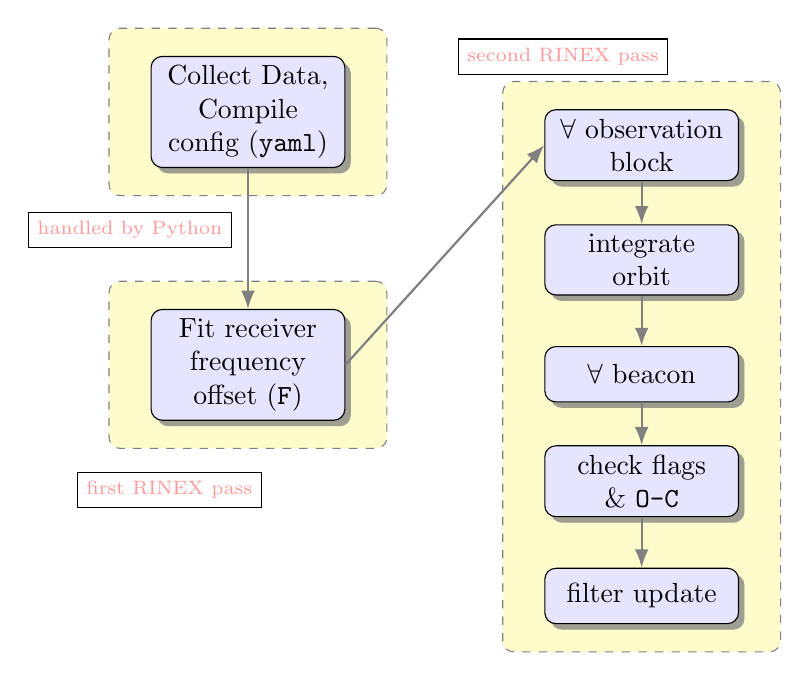
\begin{tikzpicture}
  % Draw diagram elements
  \path \etape{1}{Collect Data, Compile config (\texttt{yaml})};
  
  \path (p1.south)+(0.0, -2.5) \etape{2}{Fit receiver frequency offset (\texttt{F})};
  
  \path (p2.south)+(5.0, 3.5) \etape{3}{$\forall$ observation block};
  \path (p3.south)+(0.0,-1.0) \etape{4}{integrate orbit};
  \path (p4.south)+(0.0,-1.0) \etape{5}{$\forall$ beacon};
  \path (p5.south)+(0.0,-1.0) \etape{6}{check flags \& \texttt{O-C}};
  \path (p6.south)+(0.0,-1.0) \etape{7}{filter update};

  % Draw arrows between elements
  \path [line] (p1.south) -- node [above] {} (p2);
  \path [line] (p2.east) -- node [above] {} (p3.west);
  \path [line] (p3.south) -- node [above] {} (p4);
  \path [line] (p4.south) -- node [above] {} (p5);
  \path [line] (p5.south) -- node [above] {} (p6);
  \path [line] (p6.south) -- node [above] {} (p7);

  \begin{scope}[on background layer]
    \node (bk1) [back group] [fit=(p1)] {};
    \node (bk2) [back group] [fit=(p2)] {};
    \node (bk3) [back group] [fit=(p3) (p7)] {};
  %  \node [draw, thick, green!50!black, fill=green!75!black!25, rounded corners, fit=(p1), inner xsep=15pt, inner ysep=10pt] {};
  \end{scope}

  %\path (bk1.east)+(+6.0,0) node (ur1)[ur] {};
  %\transreceptor{bk1}{Python}{ur1}{east};
  \node[draw] at (-1.5,-1.5) {\scriptsize \textcolor{red!40}{handled by Python}};
  %\path [linepart] (#1.#4) -- node [above] {\scriptsize \textcolor{red!40}{#2}} (#3);}
  
  %\path (bk2.north)+(0.0,-4.0) node (ur2)[ur] {};
  %\transreceptor{bk2}{RINEX first pass}{ur2}{south};
  \node[draw] at (-1.0,-4.8) {\scriptsize \textcolor{red!40}{first RINEX pass}};
  \node[draw] at (4.0,+0.7) {\scriptsize \textcolor{red!40}{second RINEX pass}};

  \end{tikzpicture}
  \end{figure}
\end{frame}

\begin{frame}
  \frametitle{Current Development Focus}
    \framesubtitle{Force Model}
    \resizebox{10cm}{!}
    {
  \begin{tabular}{l|l|l}
  %\hline
    \small
    \textbf{Available} & \textbf{Update} & \textbf{Model} \\
  \hline
    Earth's gravity    & generic, v2 \& v3      & ICGEM/gfc (\cite{icgempub})\\
    Solid Earth Tides  & potential plus         & IERS 2010 \\
    (potential)        & displacement           & \\
    Ocean Tide         & potential plus         & FES2014 \\ 
    (potential)        & displacement           & (\cite{Fes2014}) \\
                       & Atmospheric Tide       & AOD1B (\cite{Dobslaw2017})\\
                       & Solid Earth Pole Tide  & IERS 2010 \\
                       & Ocean Pole Tide        & \cite{Desai2002} \\
                       & De-Aliasing            & AOD1B \\
    Third Body         &                        & JPL DE \\
    Relativity         &                        & IERS 2010 \\
    \hline
  \end{tabular}
    }
  \begin{itemize}
    \item [\textcolor{green!40}{\faExclamation}] Extensive testing against cost-g benchmark test (\cite{Lasser2020})
    \item [\textcolor{green!40}{\faExclamation}] Consistent use of Doodson numbers
    \item [\textcolor{red!40}{\faExclamation}] Identifying tidal constituents can be challenging \dots
  \end{itemize}
\end{frame}

\begin{frame}
  \frametitle{Current Development Focus}
    \framesubtitle{Force Model (Non-Conservative)}
    \resizebox{10cm}{!}
    {
  \begin{tabular}{l|l|l}
  %\hline
    \small
    \textbf{Available} & \textbf{Update} & \textbf{Model} \\
  \hline
    Atmospheric Drag   & NRLMSISE-00 to                              & \cite{nrlmsise00} \\
                       & \textcolor{blue!50}{DTM-2020}               & \cite{Bruinsma21} \\
    \textcolor{red!50}{Solar Radiation}  
                       & only direct part                            & CNES macromodel \\
    \textcolor{red!50}{Pressure} &                                   & \\
  \hline
                       & \textcolor{red!50}{Empirical Accelerations} & \\
  \end{tabular}
    }
  \begin{itemize}
    \item [\textcolor{red!40}{\faExclamation}] Generic representation of attitude
    \item [\textcolor{red!40}{\faExclamation}] Pre-processing measured attitude (\cite{Blossfeld2020})
    \item [\textcolor{red!40}{\faExclamation}] Refine SRP (albedo, CERES) \dots
    \item [\textcolor{red!40}{\faExclamation}] Hard to test
  \end{itemize}
\end{frame}

\begin{frame}
  \frametitle{Imminent Next Steps}
  \begin{itemize}[label=\textcolor{blue!40}{\textbullet}]
    \item Generic attitude representation if possible,
    \item refine SRP,
    \item revisit DORIS analysis,
    \item revisit filtering (process noise/stochastic properties)
  \end{itemize}
\end{frame}

\begin{frame}
  \frametitle{Thank you}
  \centering
  \textbf{Thank you for your attention!\\}
  %\vspace{1cm}
  \centering
  \includegraphics[width=0.1\textwidth]{gr_palaistine}

  \includegraphics[width=0.2\textwidth]{ntua}
\end{frame}

\begin{frame}[allowframebreaks]
  \frametitle{References}
    \bibliography{doris}
\end{frame}

\appendix %do not count the following slides for the total number

%\begin{frame}[plain]
%  \frametitle{Not there yet \ldots}
%\begin{figure}
%  \centering
%    \includegraphics[width=0.8\textwidth]{neweop4}
%    \caption{Conputed state Vs Sp3 results (Jason3, 02/01/2021)}
%    \label{fig:sp3-vs-mine}
%\end{figure}
%\end{frame}

\end{document}
